\documentclass[twoside]{book}

% Packages required by doxygen
\usepackage{fixltx2e}
\usepackage{calc}
\usepackage{doxygen}
\usepackage[export]{adjustbox} % also loads graphicx
\usepackage{graphicx}
\usepackage[utf8]{inputenc}
\usepackage{makeidx}
\usepackage{multicol}
\usepackage{multirow}
\PassOptionsToPackage{warn}{textcomp}
\usepackage{textcomp}
\usepackage[nointegrals]{wasysym}
\usepackage[table]{xcolor}

% Font selection
\usepackage[T1]{fontenc}
\usepackage[scaled=.90]{helvet}
\usepackage{courier}
\usepackage{amssymb}
\usepackage{sectsty}
\renewcommand{\familydefault}{\sfdefault}
\allsectionsfont{%
  \fontseries{bc}\selectfont%
  \color{darkgray}%
}
\renewcommand{\DoxyLabelFont}{%
  \fontseries{bc}\selectfont%
  \color{darkgray}%
}
\newcommand{\+}{\discretionary{\mbox{\scriptsize$\hookleftarrow$}}{}{}}

% Page & text layout
\usepackage{geometry}
\geometry{%
  a4paper,%
  top=2.5cm,%
  bottom=2.5cm,%
  left=2.5cm,%
  right=2.5cm%
}
\tolerance=750
\hfuzz=15pt
\hbadness=750
\setlength{\emergencystretch}{15pt}
\setlength{\parindent}{0cm}
\setlength{\parskip}{3ex plus 2ex minus 2ex}
\makeatletter
\renewcommand{\paragraph}{%
  \@startsection{paragraph}{4}{0ex}{-1.0ex}{1.0ex}{%
    \normalfont\normalsize\bfseries\SS@parafont%
  }%
}
\renewcommand{\subparagraph}{%
  \@startsection{subparagraph}{5}{0ex}{-1.0ex}{1.0ex}{%
    \normalfont\normalsize\bfseries\SS@subparafont%
  }%
}
\makeatother

% Headers & footers
\usepackage{fancyhdr}
\pagestyle{fancyplain}
\fancyhead[LE]{\fancyplain{}{\bfseries\thepage}}
\fancyhead[CE]{\fancyplain{}{}}
\fancyhead[RE]{\fancyplain{}{\bfseries\leftmark}}
\fancyhead[LO]{\fancyplain{}{\bfseries\rightmark}}
\fancyhead[CO]{\fancyplain{}{}}
\fancyhead[RO]{\fancyplain{}{\bfseries\thepage}}
\fancyfoot[LE]{\fancyplain{}{}}
\fancyfoot[CE]{\fancyplain{}{}}
\fancyfoot[RE]{\fancyplain{}{\bfseries\scriptsize Generated by Doxygen }}
\fancyfoot[LO]{\fancyplain{}{\bfseries\scriptsize Generated by Doxygen }}
\fancyfoot[CO]{\fancyplain{}{}}
\fancyfoot[RO]{\fancyplain{}{}}
\renewcommand{\footrulewidth}{0.4pt}
\renewcommand{\chaptermark}[1]{%
  \markboth{#1}{}%
}
\renewcommand{\sectionmark}[1]{%
  \markright{\thesection\ #1}%
}

% Indices & bibliography
\usepackage{natbib}
\usepackage[titles]{tocloft}
\setcounter{tocdepth}{3}
\setcounter{secnumdepth}{5}
\makeindex

% Hyperlinks (required, but should be loaded last)
\usepackage{ifpdf}
\ifpdf
  \usepackage[pdftex,pagebackref=true]{hyperref}
\else
  \usepackage[ps2pdf,pagebackref=true]{hyperref}
\fi
\hypersetup{%
  colorlinks=true,%
  linkcolor=blue,%
  citecolor=blue,%
  unicode%
}

% Custom commands
\newcommand{\clearemptydoublepage}{%
  \newpage{\pagestyle{empty}\cleardoublepage}%
}

\usepackage{caption}
\captionsetup{labelsep=space,justification=centering,font={bf},singlelinecheck=off,skip=4pt,position=top}

%===== C O N T E N T S =====

\begin{document}

% Titlepage & ToC
\hypersetup{pageanchor=false,
             bookmarksnumbered=true,
             pdfencoding=unicode
            }
\pagenumbering{alph}
\begin{titlepage}
\vspace*{7cm}
\begin{center}%
{\Large Compiler }\\
\vspace*{1cm}
{\large Generated by Doxygen 1.8.12}\\
\end{center}
\end{titlepage}
\clearemptydoublepage
\pagenumbering{roman}
\tableofcontents
\clearemptydoublepage
\pagenumbering{arabic}
\hypersetup{pageanchor=true}

%--- Begin generated contents ---
\chapter{Todo List}
\label{todo}
\hypertarget{todo}{}

\begin{DoxyRefList}
\item[\label{todo__todo000004}%
\hypertarget{todo__todo000004}{}%
Class \hyperlink{class_parser}{Parser} ]can use friend class to implement  
\item[\label{todo__todo000002}%
\hypertarget{todo__todo000002}{}%
Member \hyperlink{class_parser_a69a4eff828356f0c9cbf94f904ef596f}{Parser\+:\+:predictive\+Parse} ()]need test predictive\+Parse. 

solve and output Token,to set symbol\+Type and token\+Type the same only for terminal symbol.  
\item[\label{todo__todo000005}%
\hypertarget{todo__todo000005}{}%
Member \hyperlink{class_parser_a2b52de0ab06881c5f9906812aaaca3cb}{Parser\+:\+:Rec\+Des\+Parser} ]to think the relationship between the \hyperlink{class_parser}{Parser} class and Res\+Des\+Parser class 

learn and use design pattern method.  
\item[\label{todo__todo000006}%
\hypertarget{todo__todo000006}{}%
Class \hyperlink{class_rec_des_parser}{Rec\+Des\+Parser} ]finish recursive descent parser until 12-\/16 night.  
\item[\label{todo__todo000007}%
\hypertarget{todo__todo000007}{}%
Member \hyperlink{class_scanner_a377ef4e058992b4083bd835f30e113aa}{Scanner\+:\+:clean\+Up} ()]try to use try catch to solve exception.  
\item[\label{todo__todo000001}%
\hypertarget{todo__todo000001}{}%
Member \hyperlink{class_tree_node_a62f65fbb26a3d18a773f8e7f201303b3}{Tree\+Node\+:\+:Node\+Type} ]how to use c++ union 
\end{DoxyRefList}
\chapter{Bug List}
\label{bug}
\hypertarget{bug}{}

\begin{DoxyRefList}
\item[\label{bug__bug000001}%
\hypertarget{bug__bug000001}{}%
Member \hyperlink{class_scanner_aa0d88db9dafa491ffaf1c0ae92357f20}{Scanner\+:\+:next\+Token} ()]conflict with I\+D\+\_\+\+S\+T\+A\+TE 
\end{DoxyRefList}
\chapter{Namespace Index}
\section{Namespace List}
Here is a list of all documented namespaces with brief descriptions\+:\begin{DoxyCompactList}
\item\contentsline{section}{\hyperlink{namespacestd}{std} \\*Specialize std\+::less to implement user defined map. The advantage of this is that it will be picked by std\+::map \char`\"{}by default\char`\"{}, and yet you do not expose operator$<$ to client code otherwise }{\pageref{namespacestd}}{}
\end{DoxyCompactList}

\chapter{Hierarchical Index}
\section{Class Hierarchy}
This inheritance list is sorted roughly, but not completely, alphabetically\+:\begin{DoxyCompactList}
\item \contentsline{section}{A\+ST}{\pageref{class_a_s_t}}{}
\item \contentsline{section}{Error}{\pageref{class_error}}{}
\item \contentsline{section}{std\+:\+:less$<$ pair$<$ Symbol\+:\+:Symbol\+Type, Scanner\+:\+:Token\+Type $>$ $>$}{\pageref{structstd_1_1less_3_01pair_3_01_symbol_1_1_symbol_type_00_01_scanner_1_1_token_type_01_4_01_4}}{}
\item \contentsline{section}{Parser}{\pageref{class_parser}}{}
\item \contentsline{section}{Production}{\pageref{class_production}}{}
\item \contentsline{section}{Rec\+Des\+Parser}{\pageref{class_rec_des_parser}}{}
\item \contentsline{section}{Scanner}{\pageref{class_scanner}}{}
\item \contentsline{section}{Symbol}{\pageref{class_symbol}}{}
\begin{DoxyCompactList}
\item \contentsline{section}{Nonterminal\+Symbol}{\pageref{class_nonterminal_symbol}}{}
\item \contentsline{section}{Terminal\+Symbol}{\pageref{class_terminal_symbol}}{}
\end{DoxyCompactList}
\item \contentsline{section}{Scanner\+:\+:Token}{\pageref{struct_scanner_1_1_token}}{}
\item \contentsline{section}{Tree\+Node}{\pageref{class_tree_node}}{}
\end{DoxyCompactList}

\chapter{Class Index}
\section{Class List}
Here are the classes, structs, unions and interfaces with brief descriptions\+:\begin{DoxyCompactList}
\item\contentsline{section}{\hyperlink{class_a_s_t}{A\+ST} \\*Abstract syntax tree }{\pageref{class_a_s_t}}{}
\item\contentsline{section}{\hyperlink{class_error}{Error} \\*编译错误处理类 }{\pageref{class_error}}{}
\item\contentsline{section}{\hyperlink{structstd_1_1less_3_01pair_3_01_symbol_1_1_symbol_type_00_01_scanner_1_1_token_type_01_4_01_4}{std\+::less$<$ pair$<$ Symbol\+::\+Symbol\+Type, Scanner\+::\+Token\+Type $>$ $>$} }{\pageref{structstd_1_1less_3_01pair_3_01_symbol_1_1_symbol_type_00_01_scanner_1_1_token_type_01_4_01_4}}{}
\item\contentsline{section}{\hyperlink{class_nonterminal_symbol}{Nonterminal\+Symbol} }{\pageref{class_nonterminal_symbol}}{}
\item\contentsline{section}{\hyperlink{class_parser}{Parser} }{\pageref{class_parser}}{}
\item\contentsline{section}{\hyperlink{class_production}{Production} \\*Forward defined \hyperlink{class_rec_des_parser}{Rec\+Des\+Parser} }{\pageref{class_production}}{}
\item\contentsline{section}{\hyperlink{class_rec_des_parser}{Rec\+Des\+Parser} }{\pageref{class_rec_des_parser}}{}
\item\contentsline{section}{\hyperlink{class_scanner}{Scanner} \\*Scanenr class to get token from source file }{\pageref{class_scanner}}{}
\item\contentsline{section}{\hyperlink{class_symbol}{Symbol} \\*\hyperlink{class_symbol}{Symbol} class\textquotesingle{}s one \hyperlink{class_symbol}{Symbol}\textquotesingle{}s type is terminal symbol, other\textquotesingle{}s is non-\/terminal }{\pageref{class_symbol}}{}
\item\contentsline{section}{\hyperlink{class_terminal_symbol}{Terminal\+Symbol} \\*Can use override and final to manager virtual function }{\pageref{class_terminal_symbol}}{}
\item\contentsline{section}{\hyperlink{struct_scanner_1_1_token}{Scanner\+::\+Token} }{\pageref{struct_scanner_1_1_token}}{}
\item\contentsline{section}{\hyperlink{class_tree_node}{Tree\+Node} }{\pageref{class_tree_node}}{}
\end{DoxyCompactList}

\chapter{Namespace Documentation}
\hypertarget{namespacestd}{}\section{std Namespace Reference}
\label{namespacestd}\index{std@{std}}


specialize std\+::less to implement user defined map. The advantage of this is that it will be picked by std\+::map \char`\"{}by default\char`\"{}, and yet you do not expose operator$<$ to client code otherwise.  


\subsection*{Classes}
\begin{DoxyCompactItemize}
\item 
struct \hyperlink{structstd_1_1less_3_01pair_3_01_symbol_1_1_symbol_type_00_01_scanner_1_1_token_type_01_4_01_4}{less$<$ pair$<$ Symbol\+::\+Symbol\+Type, Scanner\+::\+Token\+Type $>$ $>$}
\end{DoxyCompactItemize}


\subsection{Detailed Description}
specialize std\+::less to implement user defined map. The advantage of this is that it will be picked by std\+::map \char`\"{}by default\char`\"{}, and yet you do not expose operator$<$ to client code otherwise. 
\chapter{Class Documentation}
\hypertarget{class_a_s_t}{}\section{A\+ST Class Reference}
\label{class_a_s_t}\index{A\+ST@{A\+ST}}


Abstract syntax tree.  




{\ttfamily \#include $<$A\+S\+T.\+h$>$}

\subsection*{Public Member Functions}
\begin{DoxyCompactItemize}
\item 
\hypertarget{class_a_s_t_a95385b2e90b7b4a7b407e08b74dc3b62}{}\label{class_a_s_t_a95385b2e90b7b4a7b407e08b74dc3b62} 
{\bfseries A\+ST} (const \hyperlink{class_a_s_t}{A\+ST} \&)=delete
\item 
\hypertarget{class_a_s_t_a1e7a9615a7102784cc601c946c94e9fa}{}\label{class_a_s_t_a1e7a9615a7102784cc601c946c94e9fa} 
void {\bfseries show\+A\+ST} () const
\item 
\hypertarget{class_a_s_t_a1aa227f44b3c10ff256bd070e703d98d}{}\label{class_a_s_t_a1aa227f44b3c10ff256bd070e703d98d} 
\hyperlink{class_tree_node}{Tree\+Node} $\ast$ {\bfseries get\+Root} () const
\item 
\hypertarget{class_a_s_t_ac8fd5d6840a058113abe737fa7eca302}{}\label{class_a_s_t_ac8fd5d6840a058113abe737fa7eca302} 
void {\bfseries set\+Root} (\hyperlink{class_tree_node}{Tree\+Node} $\ast$root)
\end{DoxyCompactItemize}


\subsection{Detailed Description}
Abstract syntax tree. 

The tree is used to contains all the node created in the parsing process. 

The documentation for this class was generated from the following files\+:\begin{DoxyCompactItemize}
\item 
src/A\+S\+T.\+h\item 
src/A\+S\+T.\+cpp\end{DoxyCompactItemize}

\hypertarget{class_error}{}\section{Error Class Reference}
\label{class_error}\index{Error@{Error}}


编译错误处理类  




{\ttfamily \#include $<$Error.\+h$>$}

\subsection*{Static Public Member Functions}
\begin{DoxyCompactItemize}
\item 
\hypertarget{class_error_ab109fea282348f1d8a053f6f27cb3da3}{}\label{class_error_ab109fea282348f1d8a053f6f27cb3da3} 
static void {\bfseries syntax\+Error} ()
\item 
\hypertarget{class_error_a20b415197795d362b17931d3eef70535}{}\label{class_error_a20b415197795d362b17931d3eef70535} 
static void {\bfseries number\+Error} (const string \&error)
\item 
\hypertarget{class_error_a6c43c4d14efc90e466d1bd9093f48239}{}\label{class_error_a6c43c4d14efc90e466d1bd9093f48239} 
static void {\bfseries syntax\+Error} (const string \&token\+Name, const int \&row)
\item 
\hypertarget{class_error_aced969625233c4e4db383f64c3941638}{}\label{class_error_aced969625233c4e4db383f64c3941638} 
static void {\bfseries redeclaration} (int row, string type, string name)
\item 
\hypertarget{class_error_a64d65a105dcdd097818b1d8e9240f25f}{}\label{class_error_a64d65a105dcdd097818b1d8e9240f25f} 
static void {\bfseries type\+Undeclaration} (int row, string var\+Name)
\item 
\hypertarget{class_error_a69513cd6498f5351fff9347375819175}{}\label{class_error_a69513cd6498f5351fff9347375819175} 
static void {\bfseries except\+Syntax} (const string \&error, const string \&exp) noexcept
\item 
\hypertarget{class_error_ad367940974d8904dd9ff0c1d00c7c62c}{}\label{class_error_ad367940974d8904dd9ff0c1d00c7c62c} 
static void {\bfseries syntax\+Error} (const string \&error)
\end{DoxyCompactItemize}


\subsection{Detailed Description}
编译错误处理类 

The documentation for this class was generated from the following files\+:\begin{DoxyCompactItemize}
\item 
src/Error.\+h\item 
src/Error.\+cpp\end{DoxyCompactItemize}

\hypertarget{structstd_1_1less_3_01pair_3_01_symbol_1_1_symbol_type_00_01_scanner_1_1_token_type_01_4_01_4}{}\section{std\+:\+:less$<$ pair$<$ Symbol\+:\+:Symbol\+Type, Scanner\+:\+:Token\+Type $>$ $>$ Struct Template Reference}
\label{structstd_1_1less_3_01pair_3_01_symbol_1_1_symbol_type_00_01_scanner_1_1_token_type_01_4_01_4}\index{std\+::less$<$ pair$<$ Symbol\+::\+Symbol\+Type, Scanner\+::\+Token\+Type $>$ $>$@{std\+::less$<$ pair$<$ Symbol\+::\+Symbol\+Type, Scanner\+::\+Token\+Type $>$ $>$}}
\subsection*{Public Member Functions}
\begin{DoxyCompactItemize}
\item 
\hypertarget{structstd_1_1less_3_01pair_3_01_symbol_1_1_symbol_type_00_01_scanner_1_1_token_type_01_4_01_4_a045e3f34a4fd30b0c1b362d6d255a3c4}{}\label{structstd_1_1less_3_01pair_3_01_symbol_1_1_symbol_type_00_01_scanner_1_1_token_type_01_4_01_4_a045e3f34a4fd30b0c1b362d6d255a3c4} 
bool {\bfseries operator()} (const pair$<$ \hyperlink{class_symbol_a7ee37d4cfcb980f4eddf7ed1a028da5a}{Symbol\+::\+Symbol\+Type}, \hyperlink{class_scanner_a1d588ca5cfd26bdff0e59b437da5b166}{Scanner\+::\+Token\+Type} $>$ \&lhs, const pair$<$ \hyperlink{class_symbol_a7ee37d4cfcb980f4eddf7ed1a028da5a}{Symbol\+::\+Symbol\+Type}, \hyperlink{class_scanner_a1d588ca5cfd26bdff0e59b437da5b166}{Scanner\+::\+Token\+Type} $>$ \&rhs) const
\end{DoxyCompactItemize}


The documentation for this struct was generated from the following file\+:\begin{DoxyCompactItemize}
\item 
src/Parser.\+h\end{DoxyCompactItemize}

\hypertarget{class_nonterminal_symbol}{}\section{Nonterminal\+Symbol Class Reference}
\label{class_nonterminal_symbol}\index{Nonterminal\+Symbol@{Nonterminal\+Symbol}}
Inheritance diagram for Nonterminal\+Symbol\+:\begin{figure}[H]
\begin{center}
\leavevmode
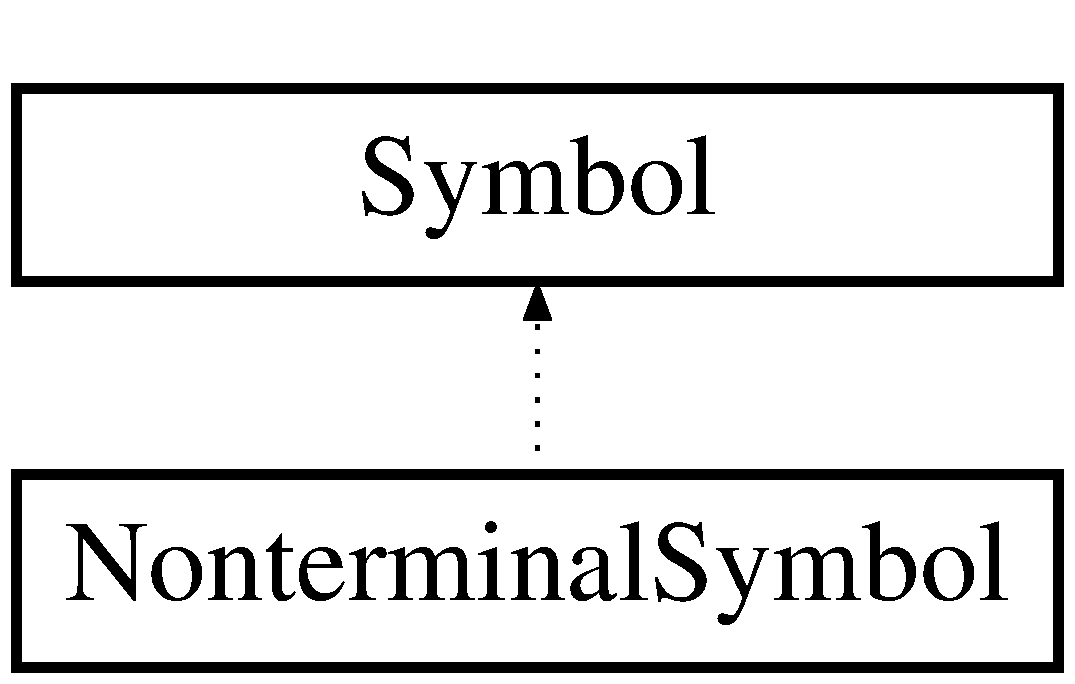
\includegraphics[height=2.000000cm]{class_nonterminal_symbol}
\end{center}
\end{figure}


The documentation for this class was generated from the following file\+:\begin{DoxyCompactItemize}
\item 
src/Symbol.\+h\end{DoxyCompactItemize}

\hypertarget{class_parser}{}\section{Parser Class Reference}
\label{class_parser}\index{Parser@{Parser}}


{\ttfamily \#include $<$Parser.\+h$>$}

\subsection*{Public Types}
\begin{DoxyCompactItemize}
\item 
\hypertarget{class_parser_a25ba9b450cd119541e982cb7c0d64d18}{}\label{class_parser_a25ba9b450cd119541e982cb7c0d64d18} 
typedef \hyperlink{class_symbol_a7ee37d4cfcb980f4eddf7ed1a028da5a}{Symbol\+::\+Symbol\+Type} {\bfseries Symtype}
\item 
using \hyperlink{class_parser_afff32ed1fe75105bdb39638ab79fbf32}{token\+Type} = \hyperlink{class_scanner_a1d588ca5cfd26bdff0e59b437da5b166}{Scanner\+::\+Token\+Type}
\item 
\hypertarget{class_parser_a965c06d2f316b898553d795e8baab9d0}{}\label{class_parser_a965c06d2f316b898553d795e8baab9d0} 
using {\bfseries Token} = \hyperlink{struct_scanner_1_1_token}{Scanner\+::\+Token}
\end{DoxyCompactItemize}
\subsection*{Public Member Functions}
\begin{DoxyCompactItemize}
\item 
\hypertarget{class_parser_a5bf0b31b43b25b002ff36068fd858f09}{}\label{class_parser_a5bf0b31b43b25b002ff36068fd858f09} 
const map$<$ pair$<$ \hyperlink{class_symbol_a7ee37d4cfcb980f4eddf7ed1a028da5a}{Symbol\+::\+Symbol\+Type}, \hyperlink{class_scanner_a1d588ca5cfd26bdff0e59b437da5b166}{Scanner\+::\+Token\+Type} $>$, \hyperlink{class_production}{Production} $>$ \& {\bfseries get\+Parser\+Table\+\_\+} () const
\item 
\hypertarget{class_parser_ae0884868884dceef40f1779a72c2e1ab}{}\label{class_parser_ae0884868884dceef40f1779a72c2e1ab} 
void {\bfseries set\+Parser\+Table\+\_\+} (const map$<$ pair$<$ \hyperlink{class_symbol_a7ee37d4cfcb980f4eddf7ed1a028da5a}{Symbol\+::\+Symbol\+Type}, \hyperlink{class_scanner_a1d588ca5cfd26bdff0e59b437da5b166}{Scanner\+::\+Token\+Type} $>$, \hyperlink{class_production}{Production} $>$ \&parser\+Table\+\_\+)
\item 
\hypertarget{class_parser_a3d06871335cd2ad61bcc7a97d969ad5c}{}\label{class_parser_a3d06871335cd2ad61bcc7a97d969ad5c} 
const \hyperlink{class_a_s_t}{A\+ST} \& {\bfseries get\+Ast\+\_\+} () const
\item 
\hypertarget{class_parser_aabf369c39918a49281118055edec57ba}{}\label{class_parser_aabf369c39918a49281118055edec57ba} 
void {\bfseries set\+Ast\+\_\+} (const \hyperlink{class_a_s_t}{A\+ST} \&ast\+\_\+)
\item 
bool \hyperlink{class_parser_a69a4eff828356f0c9cbf94f904ef596f}{predictive\+Parse} ()
\item 
void \hyperlink{class_parser_a49977242eb4dcb3ce4909d5ffbe2a813}{init\+Parser\+Table} () noexcept
\item 
\hypertarget{class_parser_af24611cf6bd9f345ce8bcc667d2220e8}{}\label{class_parser_af24611cf6bd9f345ce8bcc667d2220e8} 
void {\bfseries set\+Sourcefile} (const string \&path)
\item 
\hyperlink{struct_scanner_1_1_token}{Token} \hyperlink{class_parser_aadd9e6622f688ed2e64c0d9d1343af9c}{next\+Token} ()
\item 
void \hyperlink{class_parser_aba97a915de87d7df659a484cf8b196d8}{rollback\+Token} () noexcept(false)
\end{DoxyCompactItemize}
\subsection*{Friends}
\begin{DoxyCompactItemize}
\item 
class \hyperlink{class_parser_a2b52de0ab06881c5f9906812aaaca3cb}{Rec\+Des\+Parser}
\begin{DoxyCompactList}\small\item\em typedef and friend class. \end{DoxyCompactList}\end{DoxyCompactItemize}


\subsection{Detailed Description}
\begin{DoxyRefDesc}{Todo}
\item[\hyperlink{todo__todo000004}{Todo}]can use friend class to implement \end{DoxyRefDesc}


\subsection{Member Typedef Documentation}
\hypertarget{class_parser_afff32ed1fe75105bdb39638ab79fbf32}{}\label{class_parser_afff32ed1fe75105bdb39638ab79fbf32} 
\index{Parser@{Parser}!token\+Type@{token\+Type}}
\index{token\+Type@{token\+Type}!Parser@{Parser}}
\subsubsection{\texorpdfstring{token\+Type}{tokenType}}
{\footnotesize\ttfamily using \hyperlink{class_scanner_a1d588ca5cfd26bdff0e59b437da5b166}{Parser\+::token\+Type} =  \hyperlink{class_scanner_a1d588ca5cfd26bdff0e59b437da5b166}{Scanner\+::\+Token\+Type}}

\begin{DoxyNote}{Note}
another way to redefine type just like typedef. 
\end{DoxyNote}


\subsection{Member Function Documentation}
\hypertarget{class_parser_a49977242eb4dcb3ce4909d5ffbe2a813}{}\label{class_parser_a49977242eb4dcb3ce4909d5ffbe2a813} 
\index{Parser@{Parser}!init\+Parser\+Table@{init\+Parser\+Table}}
\index{init\+Parser\+Table@{init\+Parser\+Table}!Parser@{Parser}}
\subsubsection{\texorpdfstring{init\+Parser\+Table()}{initParserTable()}}
{\footnotesize\ttfamily void Parser\+::init\+Parser\+Table (\begin{DoxyParamCaption}{ }\end{DoxyParamCaption})\hspace{0.3cm}{\ttfamily [noexcept]}}

\begin{DoxyNote}{Note}
noexcept equal noexcept(true) this function is declared to not throw any exceptions. 
\end{DoxyNote}
\hyperlink{class_parser}{Parser} table.

E -\/ ID -\/$>$TE\textquotesingle{}

E -\/ \textquotesingle{}(\textquotesingle{}-\/$>$TE\textquotesingle{}

E\textquotesingle{} -\/ \textquotesingle{}+\textquotesingle{}$\vert$\textquotesingle{}-\/\textquotesingle{} -\/$>$+\+TE\textquotesingle{} \begin{DoxyNote}{Note}
A\+DD contains \textquotesingle{}+\textquotesingle{} and \textquotesingle{}-\/\textquotesingle{}
\end{DoxyNote}
E\textquotesingle{}-\/ \textquotesingle{})\textquotesingle{}-\/$>$ε and E\textquotesingle{} -\/ \$-\/$>$ε

T -\/ ID -\/$>$FT\textquotesingle{}

T -\/ \textquotesingle{}(\textquotesingle{}-\/$>$FT\textquotesingle{}

T\textquotesingle{} -\/ \textquotesingle{}+\textquotesingle{}$\vert$\textquotesingle{}-\/\textquotesingle{} -\/$>$ε

T\textquotesingle{} -\/ \textquotesingle{}$\ast$\textquotesingle{}$\vert$\textquotesingle{}/\textquotesingle{} -\/$>$$\ast$\+FT\textquotesingle{}

T\textquotesingle{} -\/ \textquotesingle{})\textquotesingle{}-\/$>$ε

T\textquotesingle{} -\/ \$-\/$>$ ε

F -\/ ID -\/$>$ id

F -\/ \textquotesingle{}(\textquotesingle{} -\/$>$ (E)

E -\/\+Num-\/$>$ TE\textquotesingle{}

T-\/\+Num-\/$>$ FT

F -\/\+Num-\/$>$ num; \hypertarget{class_parser_aadd9e6622f688ed2e64c0d9d1343af9c}{}\label{class_parser_aadd9e6622f688ed2e64c0d9d1343af9c} 
\index{Parser@{Parser}!next\+Token@{next\+Token}}
\index{next\+Token@{next\+Token}!Parser@{Parser}}
\subsubsection{\texorpdfstring{next\+Token()}{nextToken()}}
{\footnotesize\ttfamily \hyperlink{struct_scanner_1_1_token}{Parser\+::\+Token} Parser\+::next\+Token (\begin{DoxyParamCaption}{ }\end{DoxyParamCaption})}

local variable

set the max size of lhs\+Buffer\+\_\+ is 10. \hypertarget{class_parser_a69a4eff828356f0c9cbf94f904ef596f}{}\label{class_parser_a69a4eff828356f0c9cbf94f904ef596f} 
\index{Parser@{Parser}!predictive\+Parse@{predictive\+Parse}}
\index{predictive\+Parse@{predictive\+Parse}!Parser@{Parser}}
\subsubsection{\texorpdfstring{predictive\+Parse()}{predictiveParse()}}
{\footnotesize\ttfamily bool Parser\+::predictive\+Parse (\begin{DoxyParamCaption}{ }\end{DoxyParamCaption})}

\begin{DoxyRefDesc}{Todo}
\item[\hyperlink{todo__todo000002}{Todo}]need test predictive\+Parse. \end{DoxyRefDesc}
predicted outcome

\begin{DoxyRefDesc}{Todo}
\item[\hyperlink{todo__todo000003}{Todo}]solve and output Token,to set symbol\+Type and token\+Type the same only for terminal symbol. \end{DoxyRefDesc}


pop now.

now is non-\/terminal

find a grammar,pop now.

push symbols of \hyperlink{class_production}{Production}, last first.

solve error information.

\begin{DoxyNote}{Note}
syntax\+Error abort 
\end{DoxyNote}
\hypertarget{class_parser_aba97a915de87d7df659a484cf8b196d8}{}\label{class_parser_aba97a915de87d7df659a484cf8b196d8} 
\index{Parser@{Parser}!rollback\+Token@{rollback\+Token}}
\index{rollback\+Token@{rollback\+Token}!Parser@{Parser}}
\subsubsection{\texorpdfstring{rollback\+Token()}{rollbackToken()}}
{\footnotesize\ttfamily void Parser\+::rollback\+Token (\begin{DoxyParamCaption}{ }\end{DoxyParamCaption})\hspace{0.3cm}{\ttfamily [noexcept]}}

\begin{DoxyNote}{Note}
throw an exception. 
\end{DoxyNote}


\subsection{Friends And Related Function Documentation}
\hypertarget{class_parser_a2b52de0ab06881c5f9906812aaaca3cb}{}\label{class_parser_a2b52de0ab06881c5f9906812aaaca3cb} 
\index{Parser@{Parser}!Rec\+Des\+Parser@{Rec\+Des\+Parser}}
\index{Rec\+Des\+Parser@{Rec\+Des\+Parser}!Parser@{Parser}}
\subsubsection{\texorpdfstring{Rec\+Des\+Parser}{RecDesParser}}
{\footnotesize\ttfamily friend class \hyperlink{class_rec_des_parser}{Rec\+Des\+Parser}\hspace{0.3cm}{\ttfamily [friend]}}



typedef and friend class. 

\begin{DoxyRefDesc}{Todo}
\item[\hyperlink{todo__todo000005}{Todo}]to think the relationship between the \hyperlink{class_parser}{Parser} class and Res\+Des\+Parser class 

learn and use design pattern method. \end{DoxyRefDesc}
\begin{DoxyNote}{Note}
friend class provide interface to this class and have access to this class\textquotesingle{}s private member. 
\end{DoxyNote}


The documentation for this class was generated from the following files\+:\begin{DoxyCompactItemize}
\item 
src/Parser.\+h\item 
src/Parser.\+cpp\end{DoxyCompactItemize}

\hypertarget{class_production}{}\section{Production Class Reference}
\label{class_production}\index{Production@{Production}}


forward defined \hyperlink{class_rec_des_parser}{Rec\+Des\+Parser}  




{\ttfamily \#include $<$Parser.\+h$>$}

\subsection*{Public Member Functions}
\begin{DoxyCompactItemize}
\item 
\hypertarget{class_production_a8aacdb38e77a1a6804ac153026dd478b}{}\label{class_production_a8aacdb38e77a1a6804ac153026dd478b} 
{\bfseries Production} (const vector$<$ \hyperlink{class_symbol_a7ee37d4cfcb980f4eddf7ed1a028da5a}{Symbol\+::\+Symbol\+Type} $>$ \&grammar)
\item 
\hypertarget{class_production_acd9214af2eafdc574e67b60408931121}{}\label{class_production_acd9214af2eafdc574e67b60408931121} 
void {\bfseries add\+Symbol} (\hyperlink{class_symbol_a7ee37d4cfcb980f4eddf7ed1a028da5a}{Symbol\+::\+Symbol\+Type} symbol)
\end{DoxyCompactItemize}
\subsection*{Public Attributes}
\begin{DoxyCompactItemize}
\item 
\hypertarget{class_production_af1ba973a727cd29d8e650794ca4db609}{}\label{class_production_af1ba973a727cd29d8e650794ca4db609} 
vector$<$ \hyperlink{class_symbol_a7ee37d4cfcb980f4eddf7ed1a028da5a}{Symbol\+::\+Symbol\+Type} $>$ {\bfseries grammar}
\end{DoxyCompactItemize}


\subsection{Detailed Description}
forward defined \hyperlink{class_rec_des_parser}{Rec\+Des\+Parser} 

grammar rules class. 

The documentation for this class was generated from the following file\+:\begin{DoxyCompactItemize}
\item 
src/Parser.\+h\end{DoxyCompactItemize}

\hypertarget{class_rec_des_parser}{}\section{Rec\+Des\+Parser Class Reference}
\label{class_rec_des_parser}\index{Rec\+Des\+Parser@{Rec\+Des\+Parser}}


{\ttfamily \#include $<$Rec\+Des\+Parser.\+h$>$}

\subsection*{Static Public Member Functions}
\begin{DoxyCompactItemize}
\item 
static void \hyperlink{class_rec_des_parser_a68ff046dddb08a9cb19326c0ef619cf5}{recusive\+Descent\+Parse} (\hyperlink{class_parser}{Parser} \&parser)
\item 
static \hyperlink{class_tree_node}{Tree\+Node} $\ast$ \hyperlink{class_rec_des_parser_ae636ed876dccbbbf0df947162017ee95}{progress} (\hyperlink{class_parser}{Parser} \&parser)
\begin{DoxyCompactList}\small\item\em Progress \+:\+:= main()$<$statement\+Block$>$ \end{DoxyCompactList}\item 
static \hyperlink{class_tree_node}{Tree\+Node} $\ast$ \hyperlink{class_rec_des_parser_a80e51116fe42f872f43c351dba1b50eb}{statement\+Block} (\hyperlink{class_parser}{Parser} \&parser)
\begin{DoxyCompactList}\small\item\em statement \end{DoxyCompactList}\item 
\hypertarget{class_rec_des_parser_a2e8faf92b1c011395f75898af8b23390}{}\label{class_rec_des_parser_a2e8faf92b1c011395f75898af8b23390} 
static \hyperlink{class_tree_node}{Tree\+Node} $\ast$ \hyperlink{class_rec_des_parser_a2e8faf92b1c011395f75898af8b23390}{statements} (\hyperlink{class_parser}{Parser} \&parser)
\begin{DoxyCompactList}\small\item\em statements \+:\+:= statement \{ ;$<$statement$>$ \}; \end{DoxyCompactList}\item 
static \hyperlink{class_tree_node}{Tree\+Node} $\ast$ \hyperlink{class_rec_des_parser_a4a1fdc2b0e31b91a9e834ad60b396b37}{statement} (\hyperlink{class_parser}{Parser} \&parser)
\begin{DoxyCompactList}\small\item\em statement \+:\+:= assign\+Statement $\vert$ selection\+Statement $\vert$ loop\+Statement \end{DoxyCompactList}\item 
\hypertarget{class_rec_des_parser_a4b0ade1ab15495966a47a3445f3dc1da}{}\label{class_rec_des_parser_a4b0ade1ab15495966a47a3445f3dc1da} 
static \hyperlink{class_tree_node}{Tree\+Node} $\ast$ \hyperlink{class_rec_des_parser_a4b0ade1ab15495966a47a3445f3dc1da}{assign\+Statement} (\hyperlink{class_parser}{Parser} \&parser)
\begin{DoxyCompactList}\small\item\em assign\+Statement \+:\+:= ID \textquotesingle{}=\textquotesingle{} $<$expression$>$ \end{DoxyCompactList}\item 
\hypertarget{class_rec_des_parser_a80ce4d5f25df9d6a9311c0f3cf4b7593}{}\label{class_rec_des_parser_a80ce4d5f25df9d6a9311c0f3cf4b7593} 
static \hyperlink{class_tree_node}{Tree\+Node} $\ast$ \hyperlink{class_rec_des_parser_a80ce4d5f25df9d6a9311c0f3cf4b7593}{loop\+Statement} (\hyperlink{class_parser}{Parser} \&parser)
\begin{DoxyCompactList}\small\item\em loop\+Statement \+:\+:= do\+\_\+while\+Statement $\vert$ while\+Statement $\vert$ for\+Statement \end{DoxyCompactList}\item 
\hypertarget{class_rec_des_parser_aaccf88eb7d3084be18cbf16dc6ea10ec}{}\label{class_rec_des_parser_aaccf88eb7d3084be18cbf16dc6ea10ec} 
static \hyperlink{class_tree_node}{Tree\+Node} $\ast$ \hyperlink{class_rec_des_parser_aaccf88eb7d3084be18cbf16dc6ea10ec}{do\+\_\+while\+Statement} (\hyperlink{class_parser}{Parser} \&parser)
\begin{DoxyCompactList}\small\item\em do\+\_\+while\+Statement \+:\+:= do $<$statement\+Block$>$ while ( $<$condition$>$ ) \end{DoxyCompactList}\item 
\hypertarget{class_rec_des_parser_a76b1e2d48e0ffebb6191ad7d57ec5578}{}\label{class_rec_des_parser_a76b1e2d48e0ffebb6191ad7d57ec5578} 
static \hyperlink{class_tree_node}{Tree\+Node} $\ast$ \hyperlink{class_rec_des_parser_a76b1e2d48e0ffebb6191ad7d57ec5578}{selection\+Statement} (\hyperlink{class_parser}{Parser} \&parser)
\begin{DoxyCompactList}\small\item\em selection\+Statement \+:\+:= if ( $<$condition$>$ ) $<$statement\+Block$>$ \mbox{[}else $<$statement\+Block$>$\mbox{]} \end{DoxyCompactList}\item 
\hypertarget{class_rec_des_parser_a22fc9fb779b81433963a29055c0c26b4}{}\label{class_rec_des_parser_a22fc9fb779b81433963a29055c0c26b4} 
static \hyperlink{class_tree_node}{Tree\+Node} $\ast$ \hyperlink{class_rec_des_parser_a22fc9fb779b81433963a29055c0c26b4}{condition} (\hyperlink{class_parser}{Parser} \&parser)
\begin{DoxyCompactList}\small\item\em condition \+:\+:= $<$expression$>$ $<$relational\+Op$>$ $<$expression$>$ \end{DoxyCompactList}\item 
static \hyperlink{class_tree_node}{Tree\+Node} $\ast$ \hyperlink{class_rec_des_parser_a0640caa2edc21da4f7509a2a04c1c132}{expression} (\hyperlink{class_parser}{Parser} \&parser)
\begin{DoxyCompactList}\small\item\em expression \end{DoxyCompactList}\item 
\hypertarget{class_rec_des_parser_a68b94dd34dd185a93bd38a099ba61c97}{}\label{class_rec_des_parser_a68b94dd34dd185a93bd38a099ba61c97} 
static \hyperlink{class_tree_node}{Tree\+Node} $\ast$ \hyperlink{class_rec_des_parser_a68b94dd34dd185a93bd38a099ba61c97}{term} (\hyperlink{class_parser}{Parser} \&parser)
\begin{DoxyCompactList}\small\item\em term \+:\+:= $<$factor$>$ \{$\ast$ $<$factor$>$ $\vert$ / $<$factor$>$\} \end{DoxyCompactList}\item 
static \hyperlink{class_tree_node}{Tree\+Node} $\ast$ \hyperlink{class_rec_des_parser_ae31030c069102efd0d77aa7c187a142d}{factor} (\hyperlink{class_parser}{Parser} \&parser)
\begin{DoxyCompactList}\small\item\em factor \+:\+:= ID $\vert$ N\+UM $\vert$ (expression) \end{DoxyCompactList}\item 
static \hyperlink{class_tree_node}{Tree\+Node} $\ast$ \hyperlink{class_rec_des_parser_ab539a62bb94dce661135cebd96a45711}{num} (\hyperlink{class_parser}{Parser} \&parser)
\begin{DoxyCompactList}\small\item\em other \end{DoxyCompactList}\item 
\hypertarget{class_rec_des_parser_ae600e80953535ff51c9c5f8b0608a0f6}{}\label{class_rec_des_parser_ae600e80953535ff51c9c5f8b0608a0f6} 
static \hyperlink{class_tree_node}{Tree\+Node} $\ast$ {\bfseries id} (\hyperlink{class_parser}{Parser} \&parser)
\item 
\hypertarget{class_rec_des_parser_acfe537816711451af568ba5c4fa461cb}{}\label{class_rec_des_parser_acfe537816711451af568ba5c4fa461cb} 
static \hyperlink{class_tree_node}{Tree\+Node} $\ast$ {\bfseries relational\+Op} (\hyperlink{class_parser}{Parser} \&parser)
\end{DoxyCompactItemize}


\subsection{Detailed Description}
\begin{DoxyRefDesc}{Todo}
\item[\hyperlink{todo__todo000006}{Todo}]finish recursive descent parser until 12-\/16 night. \end{DoxyRefDesc}


\subsection{Member Function Documentation}
\hypertarget{class_rec_des_parser_a0640caa2edc21da4f7509a2a04c1c132}{}\label{class_rec_des_parser_a0640caa2edc21da4f7509a2a04c1c132} 
\index{Rec\+Des\+Parser@{Rec\+Des\+Parser}!expression@{expression}}
\index{expression@{expression}!Rec\+Des\+Parser@{Rec\+Des\+Parser}}
\subsubsection{\texorpdfstring{expression()}{expression()}}
{\footnotesize\ttfamily \hyperlink{class_tree_node}{Tree\+Node} $\ast$ Rec\+Des\+Parser\+::expression (\begin{DoxyParamCaption}\item[{\hyperlink{class_parser}{Parser} \&}]{parser }\end{DoxyParamCaption})\hspace{0.3cm}{\ttfamily [static]}}



expression 

expression \+:\+:=  \{+  $\vert$ -\/ \} \hypertarget{class_rec_des_parser_ae31030c069102efd0d77aa7c187a142d}{}\label{class_rec_des_parser_ae31030c069102efd0d77aa7c187a142d} 
\index{Rec\+Des\+Parser@{Rec\+Des\+Parser}!factor@{factor}}
\index{factor@{factor}!Rec\+Des\+Parser@{Rec\+Des\+Parser}}
\subsubsection{\texorpdfstring{factor()}{factor()}}
{\footnotesize\ttfamily \hyperlink{class_tree_node}{Tree\+Node} $\ast$ Rec\+Des\+Parser\+::factor (\begin{DoxyParamCaption}\item[{\hyperlink{class_parser}{Parser} \&}]{parser }\end{DoxyParamCaption})\hspace{0.3cm}{\ttfamily [static]}}



factor \+:\+:= ID $\vert$ N\+UM $\vert$ (expression) 

look ahead one token.

ignore the left parenthesis.

solve syntax error. \hypertarget{class_rec_des_parser_ab539a62bb94dce661135cebd96a45711}{}\label{class_rec_des_parser_ab539a62bb94dce661135cebd96a45711} 
\index{Rec\+Des\+Parser@{Rec\+Des\+Parser}!num@{num}}
\index{num@{num}!Rec\+Des\+Parser@{Rec\+Des\+Parser}}
\subsubsection{\texorpdfstring{num()}{num()}}
{\footnotesize\ttfamily \hyperlink{class_tree_node}{Tree\+Node} $\ast$ Rec\+Des\+Parser\+::num (\begin{DoxyParamCaption}\item[{\hyperlink{class_parser}{Parser} \&}]{parser }\end{DoxyParamCaption})\hspace{0.3cm}{\ttfamily [static]}}



other 

this function may throw exception.

store tmpd or tmpi in node.

rollback and syntax error. \hypertarget{class_rec_des_parser_ae636ed876dccbbbf0df947162017ee95}{}\label{class_rec_des_parser_ae636ed876dccbbbf0df947162017ee95} 
\index{Rec\+Des\+Parser@{Rec\+Des\+Parser}!progress@{progress}}
\index{progress@{progress}!Rec\+Des\+Parser@{Rec\+Des\+Parser}}
\subsubsection{\texorpdfstring{progress()}{progress()}}
{\footnotesize\ttfamily \hyperlink{class_tree_node}{Tree\+Node} $\ast$ Rec\+Des\+Parser\+::progress (\begin{DoxyParamCaption}\item[{\hyperlink{class_parser}{Parser} \&}]{parser }\end{DoxyParamCaption})\hspace{0.3cm}{\ttfamily [static]}}



Progress \+:\+:= main()$<$statement\+Block$>$ 

set the node type.

solve the syntax error.

ensure the syntax correct.

solve the syntax error. \hypertarget{class_rec_des_parser_a68ff046dddb08a9cb19326c0ef619cf5}{}\label{class_rec_des_parser_a68ff046dddb08a9cb19326c0ef619cf5} 
\index{Rec\+Des\+Parser@{Rec\+Des\+Parser}!recusive\+Descent\+Parse@{recusive\+Descent\+Parse}}
\index{recusive\+Descent\+Parse@{recusive\+Descent\+Parse}!Rec\+Des\+Parser@{Rec\+Des\+Parser}}
\subsubsection{\texorpdfstring{recusive\+Descent\+Parse()}{recusiveDescentParse()}}
{\footnotesize\ttfamily void Rec\+Des\+Parser\+::recusive\+Descent\+Parse (\begin{DoxyParamCaption}\item[{\hyperlink{class_parser}{Parser} \&}]{parser }\end{DoxyParamCaption})\hspace{0.3cm}{\ttfamily [static]}}

symbol\+: $<$ x $>$ x appear once \{ x \} x appear more than zero \mbox{[} x \mbox{]} x appear once or not appear \hypertarget{class_rec_des_parser_a4a1fdc2b0e31b91a9e834ad60b396b37}{}\label{class_rec_des_parser_a4a1fdc2b0e31b91a9e834ad60b396b37} 
\index{Rec\+Des\+Parser@{Rec\+Des\+Parser}!statement@{statement}}
\index{statement@{statement}!Rec\+Des\+Parser@{Rec\+Des\+Parser}}
\subsubsection{\texorpdfstring{statement()}{statement()}}
{\footnotesize\ttfamily \hyperlink{class_tree_node}{Tree\+Node} $\ast$ Rec\+Des\+Parser\+::statement (\begin{DoxyParamCaption}\item[{\hyperlink{class_parser}{Parser} \&}]{parser }\end{DoxyParamCaption})\hspace{0.3cm}{\ttfamily [static]}}



statement \+:\+:= assign\+Statement $\vert$ selection\+Statement $\vert$ loop\+Statement 

look ahead one token. \hypertarget{class_rec_des_parser_a80e51116fe42f872f43c351dba1b50eb}{}\label{class_rec_des_parser_a80e51116fe42f872f43c351dba1b50eb} 
\index{Rec\+Des\+Parser@{Rec\+Des\+Parser}!statement\+Block@{statement\+Block}}
\index{statement\+Block@{statement\+Block}!Rec\+Des\+Parser@{Rec\+Des\+Parser}}
\subsubsection{\texorpdfstring{statement\+Block()}{statementBlock()}}
{\footnotesize\ttfamily \hyperlink{class_tree_node}{Tree\+Node} $\ast$ Rec\+Des\+Parser\+::statement\+Block (\begin{DoxyParamCaption}\item[{\hyperlink{class_parser}{Parser} \&}]{parser }\end{DoxyParamCaption})\hspace{0.3cm}{\ttfamily [static]}}



statement 

statement\+Block \+:\+:= \textquotesingle{}\{\textquotesingle{} $<$statements$>$ \textquotesingle{}\}\textquotesingle{} ensure the syntax correct.

right parenthesis missing 

The documentation for this class was generated from the following files\+:\begin{DoxyCompactItemize}
\item 
src/Rec\+Des\+Parser.\+h\item 
src/Rec\+Des\+Parser.\+cpp\end{DoxyCompactItemize}

\hypertarget{class_scanner}{}\section{Scanner Class Reference}
\label{class_scanner}\index{Scanner@{Scanner}}


Scanenr class to get token from source file.  




{\ttfamily \#include $<$Scanner.\+h$>$}

\subsection*{Classes}
\begin{DoxyCompactItemize}
\item 
struct \hyperlink{struct_scanner_1_1_token}{Token}
\end{DoxyCompactItemize}
\subsection*{Public Types}
\begin{DoxyCompactItemize}
\item 
enum \hyperlink{class_scanner_a1d588ca5cfd26bdff0e59b437da5b166}{Token\+Type} \{ \newline
{\bfseries E\+N\+D\+O\+F\+F\+I\+LE} = 100, 
\hyperlink{class_scanner_a1d588ca5cfd26bdff0e59b437da5b166a3c7eaa7bbd93e4114909ec587d548f03}{M\+A\+IN} = 1, 
{\bfseries I\+NT} = 2, 
{\bfseries F\+L\+O\+AT} = 3, 
\newline
{\bfseries D\+O\+U\+B\+LE} = 4, 
{\bfseries C\+H\+AR} = 5, 
{\bfseries IF} = 6, 
{\bfseries E\+L\+SE} = 7, 
\newline
{\bfseries DO} = 8, 
{\bfseries W\+H\+I\+LE} = 9, 
\hyperlink{class_scanner_a1d588ca5cfd26bdff0e59b437da5b166a6cb18bf224cf14b443dde68cc98fa804}{S\+T\+R\+I\+NG} = 10, 
{\bfseries ID} = 10, 
\newline
{\bfseries B\+I\+N\+A\+R\+Y\+\_\+\+N\+U\+M\+B\+ER} = 20, 
{\bfseries D\+O\+U\+B\+L\+E\+\_\+\+N\+U\+M\+B\+ER} = 20, 
{\bfseries I\+N\+T\+\_\+\+N\+U\+M\+B\+ER} = 20, 
\hyperlink{class_scanner_a1d588ca5cfd26bdff0e59b437da5b166a92075cf0b9bcb96f062e94a3b84c6c73}{A\+DD} = 22, 
\newline
{\bfseries A\+S\+S\+I\+GN} = 21, 
{\bfseries S\+UB} = 23, 
{\bfseries M\+U\+LT} = 24, 
{\bfseries D\+IV} = 25, 
\newline
{\bfseries L\+E\+F\+T\+\_\+\+P\+AR} = 26, 
{\bfseries R\+I\+G\+H\+T\+\_\+\+P\+AR} = 27, 
{\bfseries L\+E\+F\+T\+\_\+\+B\+L\+O\+CK} = 28, 
{\bfseries R\+I\+G\+H\+T\+\_\+\+B\+L\+O\+CK} = 29, 
\newline
{\bfseries C\+O\+M\+MA} = 30, 
{\bfseries S\+E\+M\+I\+C\+O\+L\+ON} = 31, 
{\bfseries G\+R\+E\+A\+T\+ER} = 32, 
{\bfseries G\+R\+E\+A\+T\+E\+R\+\_\+\+E\+Q\+U\+AL} = 33, 
\newline
{\bfseries S\+M\+A\+L\+L\+ER} = 34, 
{\bfseries S\+M\+A\+L\+L\+E\+R\+\_\+\+E\+Q\+U\+AL} = 35, 
{\bfseries E\+Q\+U\+AL} = 36, 
{\bfseries N\+O\+N\+\_\+\+E\+Q\+U\+AL} = 37, 
\newline
{\bfseries H\+A\+S\+H\+\_\+\+M\+A\+RK} = 38, 
{\bfseries B\+O\+OL} = 39, 
\hyperlink{class_scanner_a1d588ca5cfd26bdff0e59b437da5b166a57fa4cabbebd964ade8ea1ca070ac7b4}{K\+E\+Y\+\_\+\+W\+O\+RD} = 50, 
{\bfseries S\+Y\+M\+B\+OL} = 51, 
\newline
{\bfseries N\+O\+NE} = 52, 
{\bfseries E\+R\+R\+OR} = 53, 
{\bfseries E\+N\+D\+\_\+\+M\+A\+RK} = 100
 \}
\end{DoxyCompactItemize}
\subsection*{Public Member Functions}
\begin{DoxyCompactItemize}
\item 
void \hyperlink{class_scanner_a299d27000feef9ce880a69486d6e67d2}{init\+Key\+Words} ()
\item 
\hypertarget{class_scanner_aa984b69f762727024ffa36bc6171c2c2}{}\label{class_scanner_aa984b69f762727024ffa36bc6171c2c2} 
void {\bfseries init\+Symbols} ()
\item 
\hypertarget{class_scanner_a2a0ebb604a33fae2792df2fe8e0f3354}{}\label{class_scanner_a2a0ebb604a33fae2792df2fe8e0f3354} 
void {\bfseries open\+File} (const string \&filename)
\item 
\hypertarget{class_scanner_a3cd96a9a11c56790e5c053129b9bd8ad}{}\label{class_scanner_a3cd96a9a11c56790e5c053129b9bd8ad} 
void {\bfseries close\+File} ()
\item 
\hyperlink{struct_scanner_1_1_token}{Token} \hyperlink{class_scanner_aa0d88db9dafa491ffaf1c0ae92357f20}{next\+Token} ()
\item 
\hypertarget{class_scanner_a0742be27da7d62b413b6214f8a8b1621}{}\label{class_scanner_a0742be27da7d62b413b6214f8a8b1621} 
unsigned int {\bfseries get\+Row} ()
\item 
\hypertarget{class_scanner_ac8a97e1e2bd21cf929c99f498842dad5}{}\label{class_scanner_ac8a97e1e2bd21cf929c99f498842dad5} 
string {\bfseries get\+Line\+Buffer} ()
\item 
\hypertarget{class_scanner_a70814f701d44836c2b6e1ca704ce1bb3}{}\label{class_scanner_a70814f701d44836c2b6e1ca704ce1bb3} 
void {\bfseries reset\+Row} ()
\item 
void \hyperlink{class_scanner_a377ef4e058992b4083bd835f30e113aa}{clean\+Up} ()
\end{DoxyCompactItemize}
\subsection*{Public Attributes}
\begin{DoxyCompactItemize}
\item 
\hypertarget{class_scanner_abef0898a8940e74a01194f3f249641c9}{}\label{class_scanner_abef0898a8940e74a01194f3f249641c9} 
set$<$ string $>$ {\bfseries key\+Words}
\item 
\hypertarget{class_scanner_ae575d45434a167e925691c6fca90805b}{}\label{class_scanner_ae575d45434a167e925691c6fca90805b} 
set$<$ string $>$ {\bfseries symbols}
\end{DoxyCompactItemize}


\subsection{Detailed Description}
Scanenr class to get token from source file. 

\subsection{Member Enumeration Documentation}
\hypertarget{class_scanner_a1d588ca5cfd26bdff0e59b437da5b166}{}\label{class_scanner_a1d588ca5cfd26bdff0e59b437da5b166} 
\index{Scanner@{Scanner}!Token\+Type@{Token\+Type}}
\index{Token\+Type@{Token\+Type}!Scanner@{Scanner}}
\subsubsection{\texorpdfstring{Token\+Type}{TokenType}}
{\footnotesize\ttfamily enum \hyperlink{class_scanner_a1d588ca5cfd26bdff0e59b437da5b166}{Scanner\+::\+Token\+Type}}

\begin{DoxyNote}{Note}
explicit define the enum type value. 
\end{DoxyNote}
\begin{DoxyEnumFields}{Enumerator}
\raisebox{\heightof{T}}[0pt][0pt]{\index{M\+A\+IN@{M\+A\+IN}!Scanner@{Scanner}}\index{Scanner@{Scanner}!M\+A\+IN@{M\+A\+IN}}}\hypertarget{class_scanner_a1d588ca5cfd26bdff0e59b437da5b166a3c7eaa7bbd93e4114909ec587d548f03}{}\label{class_scanner_a1d588ca5cfd26bdff0e59b437da5b166a3c7eaa7bbd93e4114909ec587d548f03} 
M\+A\+IN&terminal symbol key word \\
\hline

\raisebox{\heightof{T}}[0pt][0pt]{\index{S\+T\+R\+I\+NG@{S\+T\+R\+I\+NG}!Scanner@{Scanner}}\index{Scanner@{Scanner}!S\+T\+R\+I\+NG@{S\+T\+R\+I\+NG}}}\hypertarget{class_scanner_a1d588ca5cfd26bdff0e59b437da5b166a6cb18bf224cf14b443dde68cc98fa804}{}\label{class_scanner_a1d588ca5cfd26bdff0e59b437da5b166a6cb18bf224cf14b443dde68cc98fa804} 
S\+T\+R\+I\+NG&variable \\
\hline

\raisebox{\heightof{T}}[0pt][0pt]{\index{A\+DD@{A\+DD}!Scanner@{Scanner}}\index{Scanner@{Scanner}!A\+DD@{A\+DD}}}\hypertarget{class_scanner_a1d588ca5cfd26bdff0e59b437da5b166a92075cf0b9bcb96f062e94a3b84c6c73}{}\label{class_scanner_a1d588ca5cfd26bdff0e59b437da5b166a92075cf0b9bcb96f062e94a3b84c6c73} 
A\+DD&symboL \\
\hline

\raisebox{\heightof{T}}[0pt][0pt]{\index{K\+E\+Y\+\_\+\+W\+O\+RD@{K\+E\+Y\+\_\+\+W\+O\+RD}!Scanner@{Scanner}}\index{Scanner@{Scanner}!K\+E\+Y\+\_\+\+W\+O\+RD@{K\+E\+Y\+\_\+\+W\+O\+RD}}}\hypertarget{class_scanner_a1d588ca5cfd26bdff0e59b437da5b166a57fa4cabbebd964ade8ea1ca070ac7b4}{}\label{class_scanner_a1d588ca5cfd26bdff0e59b437da5b166a57fa4cabbebd964ade8ea1ca070ac7b4} 
K\+E\+Y\+\_\+\+W\+O\+RD&T\+OP symbol. \\
\hline

\end{DoxyEnumFields}


\subsection{Member Function Documentation}
\hypertarget{class_scanner_a377ef4e058992b4083bd835f30e113aa}{}\label{class_scanner_a377ef4e058992b4083bd835f30e113aa} 
\index{Scanner@{Scanner}!clean\+Up@{clean\+Up}}
\index{clean\+Up@{clean\+Up}!Scanner@{Scanner}}
\subsubsection{\texorpdfstring{clean\+Up()}{cleanUp()}}
{\footnotesize\ttfamily void Scanner\+::clean\+Up (\begin{DoxyParamCaption}{ }\end{DoxyParamCaption})}

\begin{DoxyRefDesc}{Todo}
\item[\hyperlink{todo__todo000007}{Todo}]try to use try catch to solve exception. \end{DoxyRefDesc}
\hypertarget{class_scanner_a299d27000feef9ce880a69486d6e67d2}{}\label{class_scanner_a299d27000feef9ce880a69486d6e67d2} 
\index{Scanner@{Scanner}!init\+Key\+Words@{init\+Key\+Words}}
\index{init\+Key\+Words@{init\+Key\+Words}!Scanner@{Scanner}}
\subsubsection{\texorpdfstring{init\+Key\+Words()}{initKeyWords()}}
{\footnotesize\ttfamily void Scanner\+::init\+Key\+Words (\begin{DoxyParamCaption}{ }\end{DoxyParamCaption})}

\begin{DoxyNote}{Note}
to use initialize\+\_\+list key\+Words.\+clear(); key\+Words.\+insert(\char`\"{}int\char`\"{}); key\+Words.\+insert(\char`\"{}printf\char`\"{}); key\+Words.\+insert(\char`\"{}void\char`\"{}); key\+Words.\+insert(\char`\"{}if\char`\"{}); key\+Words.\+insert(\char`\"{}else\char`\"{}); key\+Words.\+insert(\char`\"{}else if\char`\"{}); key\+Words.\+insert(\char`\"{}return\char`\"{}); key\+Words.\+insert(\char`\"{}while\char`\"{}); key\+Words.\+insert(\char`\"{}break\char`\"{}); key\+Words.\+insert(\char`\"{}do\char`\"{}); key\+Words.\+insert(\char`\"{}for\char`\"{});
\end{DoxyNote}
\hypertarget{class_scanner_aa0d88db9dafa491ffaf1c0ae92357f20}{}\label{class_scanner_aa0d88db9dafa491ffaf1c0ae92357f20} 
\index{Scanner@{Scanner}!next\+Token@{next\+Token}}
\index{next\+Token@{next\+Token}!Scanner@{Scanner}}
\subsubsection{\texorpdfstring{next\+Token()}{nextToken()}}
{\footnotesize\ttfamily \hyperlink{struct_scanner_1_1_token}{Scanner\+::\+Token} Scanner\+::next\+Token (\begin{DoxyParamCaption}{ }\end{DoxyParamCaption})}

\begin{DoxyRefDesc}{Bug}
\item[\hyperlink{bug__bug000001}{Bug}]conflict with I\+D\+\_\+\+S\+T\+A\+TE \end{DoxyRefDesc}


The documentation for this class was generated from the following files\+:\begin{DoxyCompactItemize}
\item 
src/Scanner.\+h\item 
src/Scanner.\+cpp\end{DoxyCompactItemize}

\hypertarget{class_symbol}{}\section{Symbol Class Reference}
\label{class_symbol}\index{Symbol@{Symbol}}


\hyperlink{class_symbol}{Symbol} class\textquotesingle{}s one \hyperlink{class_symbol}{Symbol}\textquotesingle{}s type is terminal symbol, other\textquotesingle{}s is non-\/terminal.  




{\ttfamily \#include $<$Symbol.\+h$>$}

Inheritance diagram for Symbol\+:\begin{figure}[H]
\begin{center}
\leavevmode
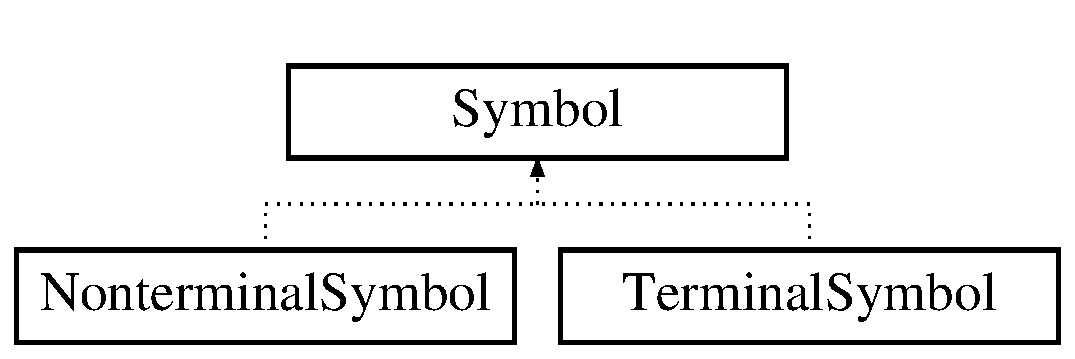
\includegraphics[height=2.000000cm]{class_symbol}
\end{center}
\end{figure}
\subsection*{Public Types}
\begin{DoxyCompactItemize}
\item 
enum \hyperlink{class_symbol_a7ee37d4cfcb980f4eddf7ed1a028da5a}{Symbol\+Type} \{ \newline
{\bfseries primary\+\_\+expression}, 
\hyperlink{class_symbol_a7ee37d4cfcb980f4eddf7ed1a028da5aa8661510d8a27e67fc96161d1c67289bd}{expression}, 
{\bfseries expression\+\_\+}, 
{\bfseries multiplicative\+\_\+expression}, 
\newline
{\bfseries multiplicative\+\_\+expression\+\_\+}, 
{\bfseries additive\+\_\+expression}, 
{\bfseries relational\+\_\+expression}, 
{\bfseries equality\+\_\+expression}, 
\newline
{\bfseries assignment\+\_\+expression}, 
\hyperlink{class_symbol_a7ee37d4cfcb980f4eddf7ed1a028da5aa3db3ca894c8b0c7c2a94e4bef890032b}{additive\+\_\+operator} = 22, 
{\bfseries multiplicative\+\_\+operator} = 24, 
{\bfseries assignment\+\_\+operator} = 21, 
\newline
{\bfseries terminal\+\_\+id} = 10, 
{\bfseries terminal\+\_\+num} = 20, 
{\bfseries terminal\+\_\+double} = 20, 
{\bfseries terminal\+\_\+add} = 22, 
\newline
{\bfseries terminal\+\_\+sub} = 23, 
{\bfseries terminal\+\_\+mult} = 24, 
{\bfseries terminal\+\_\+div} = 25, 
{\bfseries terminal\+\_\+leftpar} = 26, 
\newline
{\bfseries terminal\+\_\+rightpar} = 27, 
{\bfseries terminal\+\_\+leftblock} = 28, 
{\bfseries terminal\+\_\+rightblock} = 29, 
{\bfseries terminal\+\_\+comma} = 30, 
\newline
{\bfseries terminal\+\_\+semincolon} = 31, 
{\bfseries terminal\+\_\+greater} = 32, 
{\bfseries terminal\+\_\+end} = 100, 
{\bfseries terminal\+\_\+ε}
 \}
\end{DoxyCompactItemize}
\subsection*{Public Member Functions}
\begin{DoxyCompactItemize}
\item 
\hypertarget{class_symbol_aaea83d504a1096a6452d4da0d22a6cf2}{}\label{class_symbol_aaea83d504a1096a6452d4da0d22a6cf2} 
{\bfseries Symbol} (bool is\+Terminal)
\end{DoxyCompactItemize}
\subsection*{Static Public Member Functions}
\begin{DoxyCompactItemize}
\item 
\hypertarget{class_symbol_a9a898baa9dd070590594f294335d9125}{}\label{class_symbol_a9a898baa9dd070590594f294335d9125} 
static bool {\bfseries isterminal} (\hyperlink{class_symbol_a7ee37d4cfcb980f4eddf7ed1a028da5a}{Symbol\+Type} type)
\end{DoxyCompactItemize}
\subsection*{Public Attributes}
\begin{DoxyCompactItemize}
\item 
\hypertarget{class_symbol_a7911a477f0959199fd61fb6a37fb5397}{}\label{class_symbol_a7911a477f0959199fd61fb6a37fb5397} 
bool {\bfseries is\+Terminal}
\end{DoxyCompactItemize}


\subsection{Detailed Description}
\hyperlink{class_symbol}{Symbol} class\textquotesingle{}s one \hyperlink{class_symbol}{Symbol}\textquotesingle{}s type is terminal symbol, other\textquotesingle{}s is non-\/terminal. 

\subsection{Member Enumeration Documentation}
\hypertarget{class_symbol_a7ee37d4cfcb980f4eddf7ed1a028da5a}{}\label{class_symbol_a7ee37d4cfcb980f4eddf7ed1a028da5a} 
\index{Symbol@{Symbol}!Symbol\+Type@{Symbol\+Type}}
\index{Symbol\+Type@{Symbol\+Type}!Symbol@{Symbol}}
\subsubsection{\texorpdfstring{Symbol\+Type}{SymbolType}}
{\footnotesize\ttfamily enum \hyperlink{class_symbol_a7ee37d4cfcb980f4eddf7ed1a028da5a}{Symbol\+::\+Symbol\+Type}}

\begin{DoxyNote}{Note}
the enum type value can\textquotesingle{}t the same. 
\end{DoxyNote}
\begin{DoxyEnumFields}{Enumerator}
\raisebox{\heightof{T}}[0pt][0pt]{\index{expression@{expression}!Symbol@{Symbol}}\index{Symbol@{Symbol}!expression@{expression}}}\hypertarget{class_symbol_a7ee37d4cfcb980f4eddf7ed1a028da5aa8661510d8a27e67fc96161d1c67289bd}{}\label{class_symbol_a7ee37d4cfcb980f4eddf7ed1a028da5aa8661510d8a27e67fc96161d1c67289bd} 
expression&-\/-\/---0 \\
\hline

\raisebox{\heightof{T}}[0pt][0pt]{\index{additive\+\_\+operator@{additive\+\_\+operator}!Symbol@{Symbol}}\index{Symbol@{Symbol}!additive\+\_\+operator@{additive\+\_\+operator}}}\hypertarget{class_symbol_a7ee37d4cfcb980f4eddf7ed1a028da5aa3db3ca894c8b0c7c2a94e4bef890032b}{}\label{class_symbol_a7ee37d4cfcb980f4eddf7ed1a028da5aa3db3ca894c8b0c7c2a94e4bef890032b} 
additive\+\_\+operator&-\/---8 Non-\/terminal symbol limit. \\
\hline

\end{DoxyEnumFields}


The documentation for this class was generated from the following files\+:\begin{DoxyCompactItemize}
\item 
src/Symbol.\+h\item 
src/Symbol.\+cpp\end{DoxyCompactItemize}

\hypertarget{class_terminal_symbol}{}\section{Terminal\+Symbol Class Reference}
\label{class_terminal_symbol}\index{Terminal\+Symbol@{Terminal\+Symbol}}


can use override and final to manager virtual function.  




{\ttfamily \#include $<$Symbol.\+h$>$}

Inheritance diagram for Terminal\+Symbol\+:\begin{figure}[H]
\begin{center}
\leavevmode
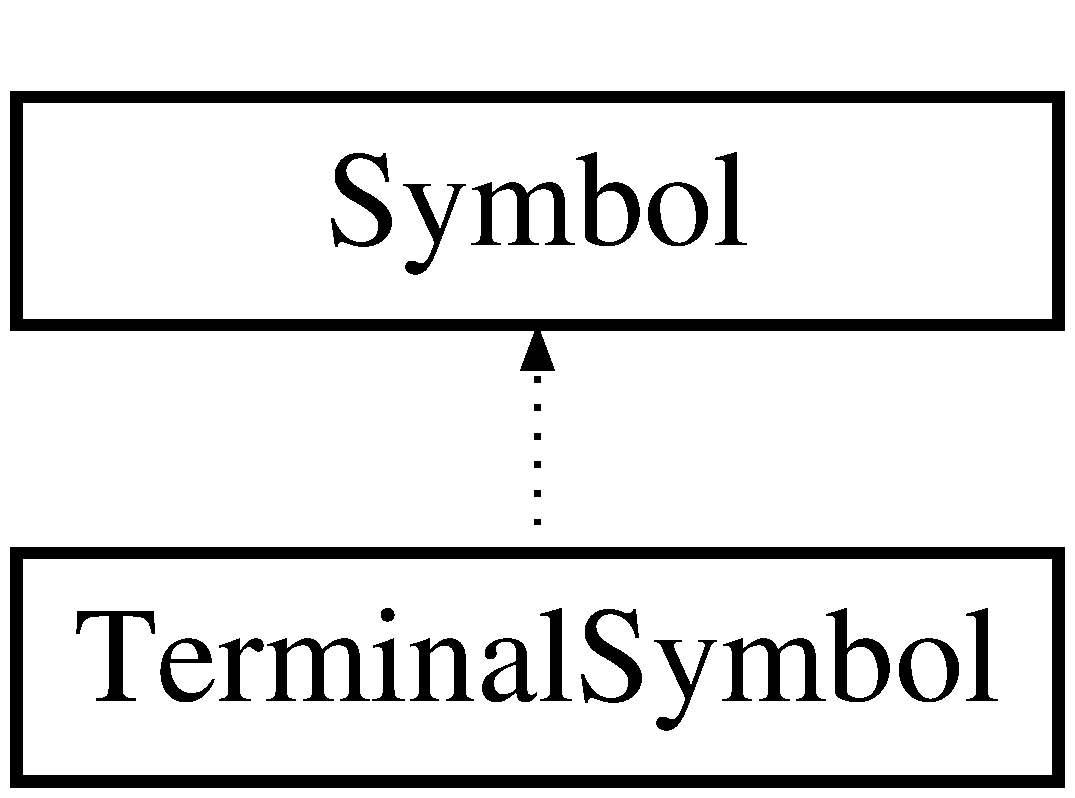
\includegraphics[height=2.000000cm]{class_terminal_symbol}
\end{center}
\end{figure}


\subsection{Detailed Description}
can use override and final to manager virtual function. 

The documentation for this class was generated from the following file\+:\begin{DoxyCompactItemize}
\item 
src/Symbol.\+h\end{DoxyCompactItemize}

\hypertarget{struct_scanner_1_1_token}{}\section{Scanner\+:\+:Token Struct Reference}
\label{struct_scanner_1_1_token}\index{Scanner\+::\+Token@{Scanner\+::\+Token}}
\subsection*{Public Attributes}
\begin{DoxyCompactItemize}
\item 
\hypertarget{struct_scanner_1_1_token_ac1231a1f9706c2fef3c67ca8670d0174}{}\label{struct_scanner_1_1_token_ac1231a1f9706c2fef3c67ca8670d0174} 
\hyperlink{class_scanner_a1d588ca5cfd26bdff0e59b437da5b166}{Token\+Type} {\bfseries kind}
\item 
\hypertarget{struct_scanner_1_1_token_a5a234137ce0843189e909f7146945efe}{}\label{struct_scanner_1_1_token_a5a234137ce0843189e909f7146945efe} 
string {\bfseries lexeme}
\item 
\hypertarget{struct_scanner_1_1_token_af83dcc1337613ad1c8d80aec9d8123bb}{}\label{struct_scanner_1_1_token_af83dcc1337613ad1c8d80aec9d8123bb} 
unsigned int {\bfseries row}
\item 
\hypertarget{struct_scanner_1_1_token_a0f0616aadf99dfa1707c6beee4c7453c}{}\label{struct_scanner_1_1_token_a0f0616aadf99dfa1707c6beee4c7453c} 
unsigned int {\bfseries pos}
\end{DoxyCompactItemize}


The documentation for this struct was generated from the following file\+:\begin{DoxyCompactItemize}
\item 
src/Scanner.\+h\end{DoxyCompactItemize}

\hypertarget{class_tree_node}{}\section{Tree\+Node Class Reference}
\label{class_tree_node}\index{Tree\+Node@{Tree\+Node}}
\subsection*{Public Types}
\begin{DoxyCompactItemize}
\item 
enum \hyperlink{class_tree_node_a62f65fbb26a3d18a773f8e7f201303b3}{Node\+Type} \{ \newline
{\bfseries E\+N\+D\+O\+F\+F\+I\+LE} = 100, 
\hyperlink{class_tree_node_a62f65fbb26a3d18a773f8e7f201303b3a8fe6cd5b7bb583a57703ed4083cd55fa}{M\+A\+IN} = 1, 
{\bfseries I\+NT} = 2, 
{\bfseries F\+L\+O\+AT} = 3, 
\newline
{\bfseries D\+O\+U\+B\+LE} = 4, 
{\bfseries C\+H\+AR} = 5, 
{\bfseries IF} = 6, 
{\bfseries E\+L\+SE} = 7, 
\newline
{\bfseries DO} = 8, 
{\bfseries W\+H\+I\+LE} = 9, 
\hyperlink{class_tree_node_a62f65fbb26a3d18a773f8e7f201303b3a8526948dee4855c6ea6d49dca25b79ff}{S\+T\+R\+I\+NG} = 10, 
{\bfseries ID} = 10, 
\newline
{\bfseries B\+I\+N\+A\+R\+Y\+\_\+\+N\+U\+M\+B\+ER} = 20, 
{\bfseries D\+O\+U\+B\+L\+E\+\_\+\+N\+U\+M\+B\+ER} = 20, 
{\bfseries I\+N\+T\+\_\+\+N\+U\+M\+B\+ER} = 20, 
\hyperlink{class_tree_node_a62f65fbb26a3d18a773f8e7f201303b3a8c682e3267299864062c35947b16776f}{A\+DD} = 22, 
\newline
{\bfseries A\+S\+S\+I\+GN} = 21, 
{\bfseries S\+UB} = 23, 
{\bfseries M\+U\+LT} = 24, 
{\bfseries D\+IV} = 25, 
\newline
{\bfseries L\+E\+F\+T\+\_\+\+P\+AR} = 26, 
{\bfseries R\+I\+G\+H\+T\+\_\+\+P\+AR} = 27, 
{\bfseries L\+E\+F\+T\+\_\+\+B\+L\+O\+CK} = 28, 
{\bfseries R\+I\+G\+H\+T\+\_\+\+B\+L\+O\+CK} = 29, 
\newline
{\bfseries C\+O\+M\+MA} = 30, 
{\bfseries S\+E\+M\+I\+C\+O\+L\+ON} = 31, 
{\bfseries G\+R\+E\+A\+T\+ER} = 32, 
{\bfseries G\+R\+E\+A\+T\+E\+R\+\_\+\+E\+Q\+U\+AL} = 33, 
\newline
{\bfseries S\+M\+A\+L\+L\+ER} = 34, 
{\bfseries S\+M\+A\+L\+L\+E\+R\+\_\+\+E\+Q\+U\+AL} = 35, 
{\bfseries E\+Q\+U\+AL} = 36, 
{\bfseries N\+O\+N\+\_\+\+E\+Q\+U\+AL} = 37, 
\newline
{\bfseries H\+A\+S\+H\+\_\+\+M\+A\+RK} = 38, 
{\bfseries B\+O\+OL} = 39, 
\hyperlink{class_tree_node_a62f65fbb26a3d18a773f8e7f201303b3aefb73e7c0ba3285bb50361872831df9e}{K\+E\+Y\+\_\+\+W\+O\+RD} = 50, 
{\bfseries S\+Y\+M\+B\+OL} = 51, 
\newline
{\bfseries N\+O\+NE} = 52, 
{\bfseries E\+R\+R\+OR} = 53, 
{\bfseries E\+N\+D\+\_\+\+M\+A\+RK} = 100, 
\hyperlink{class_tree_node_a62f65fbb26a3d18a773f8e7f201303b3acbe0968aaa30775f92a934bdf318dcf9}{P\+R\+O\+G\+R\+E\+SS}, 
\newline
{\bfseries S\+T\+A\+T\+E\+M\+E\+NT}, 
{\bfseries S\+T\+A\+T\+E\+M\+E\+N\+TS}, 
{\bfseries S\+T\+A\+T\+E\+M\+E\+N\+T\+\_\+\+B\+L\+O\+CK}, 
{\bfseries A\+S\+S\+I\+G\+N\+\_\+\+S\+T\+A\+T\+E\+M\+E\+NT}, 
\newline
{\bfseries D\+O\+\_\+\+W\+H\+I\+L\+E\+\_\+\+S\+T\+A\+T\+E\+M\+E\+NT}, 
{\bfseries I\+F\+\_\+\+S\+T\+A\+T\+E\+M\+E\+NT}, 
{\bfseries E\+L\+S\+E\+\_\+\+S\+T\+A\+T\+E\+M\+E\+NT}
 \}
\end{DoxyCompactItemize}
\subsection*{Public Member Functions}
\begin{DoxyCompactItemize}
\item 
const std\+::vector$<$ \hyperlink{class_tree_node}{Tree\+Node} $\ast$ $>$ \& \hyperlink{class_tree_node_a8baa49dd046d1365dc85c85f12beda79}{get\+Children\+\_\+} () const
\begin{DoxyCompactList}\small\item\em Node get\+Children method. \end{DoxyCompactList}\item 
\hypertarget{class_tree_node_aeff1bea5b97d0127d21c3e852aaff74e}{}\label{class_tree_node_aeff1bea5b97d0127d21c3e852aaff74e} 
void \hyperlink{class_tree_node_aeff1bea5b97d0127d21c3e852aaff74e}{set\+Children\+\_\+} (const std\+::vector$<$ \hyperlink{class_tree_node}{Tree\+Node} $\ast$$>$ \&children\+\_\+)
\begin{DoxyCompactList}\small\item\em Node set\+Children method. \end{DoxyCompactList}\item 
\hypertarget{class_tree_node_a6b1c9937781afd0acae55b610a5c327c}{}\label{class_tree_node_a6b1c9937781afd0acae55b610a5c327c} 
void {\bfseries add\+Child} (\hyperlink{class_tree_node}{Tree\+Node} $\ast$child)
\item 
\hypertarget{class_tree_node_aa8d8232a5c5d23bcfb9ee9ff2515eaad}{}\label{class_tree_node_aa8d8232a5c5d23bcfb9ee9ff2515eaad} 
void {\bfseries show\+Node} ()
\end{DoxyCompactItemize}
\subsection*{Public Attributes}
\begin{DoxyCompactItemize}
\item 
\hypertarget{class_tree_node_a303725338fb06e7b9af7399e49d0349c}{}\label{class_tree_node_a303725338fb06e7b9af7399e49d0349c} 
int \hyperlink{class_tree_node_a303725338fb06e7b9af7399e49d0349c}{deep} \{0\}
\begin{DoxyCompactList}\small\item\em node\textquotesingle{}s level. \end{DoxyCompactList}\item 
\hypertarget{class_tree_node_a226b9c8f9092850e587a187bca0766f5}{}\label{class_tree_node_a226b9c8f9092850e587a187bca0766f5} 
bool {\bfseries terminal} \{false\}
\item 
\hypertarget{class_tree_node_a0356b323f5d3e9cb2d393d439771af15}{}\label{class_tree_node_a0356b323f5d3e9cb2d393d439771af15} 
enum \hyperlink{class_tree_node_a62f65fbb26a3d18a773f8e7f201303b3}{Tree\+Node\+::\+Node\+Type} {\bfseries kind}
\item 
\hypertarget{class_tree_node_a7bb7b4103a78bb399d7ed87c2f406ae3}{}\label{class_tree_node_a7bb7b4103a78bb399d7ed87c2f406ae3} 
\hyperlink{struct_scanner_1_1_token}{Scanner\+::\+Token} {\bfseries token}
\end{DoxyCompactItemize}


\subsection{Member Enumeration Documentation}
\hypertarget{class_tree_node_a62f65fbb26a3d18a773f8e7f201303b3}{}\label{class_tree_node_a62f65fbb26a3d18a773f8e7f201303b3} 
\index{Tree\+Node@{Tree\+Node}!Node\+Type@{Node\+Type}}
\index{Node\+Type@{Node\+Type}!Tree\+Node@{Tree\+Node}}
\subsubsection{\texorpdfstring{Node\+Type}{NodeType}}
{\footnotesize\ttfamily enum \hyperlink{class_tree_node_a62f65fbb26a3d18a773f8e7f201303b3}{Tree\+Node\+::\+Node\+Type}}

\begin{DoxyRefDesc}{Todo}
\item[\hyperlink{todo__todo000001}{Todo}]how to use c++ union \end{DoxyRefDesc}
\begin{DoxyEnumFields}{Enumerator}
\raisebox{\heightof{T}}[0pt][0pt]{\index{M\+A\+IN@{M\+A\+IN}!Tree\+Node@{Tree\+Node}}\index{Tree\+Node@{Tree\+Node}!M\+A\+IN@{M\+A\+IN}}}\hypertarget{class_tree_node_a62f65fbb26a3d18a773f8e7f201303b3a8fe6cd5b7bb583a57703ed4083cd55fa}{}\label{class_tree_node_a62f65fbb26a3d18a773f8e7f201303b3a8fe6cd5b7bb583a57703ed4083cd55fa} 
M\+A\+IN&terminal symbol key word \\
\hline

\raisebox{\heightof{T}}[0pt][0pt]{\index{S\+T\+R\+I\+NG@{S\+T\+R\+I\+NG}!Tree\+Node@{Tree\+Node}}\index{Tree\+Node@{Tree\+Node}!S\+T\+R\+I\+NG@{S\+T\+R\+I\+NG}}}\hypertarget{class_tree_node_a62f65fbb26a3d18a773f8e7f201303b3a8526948dee4855c6ea6d49dca25b79ff}{}\label{class_tree_node_a62f65fbb26a3d18a773f8e7f201303b3a8526948dee4855c6ea6d49dca25b79ff} 
S\+T\+R\+I\+NG&variable \\
\hline

\raisebox{\heightof{T}}[0pt][0pt]{\index{A\+DD@{A\+DD}!Tree\+Node@{Tree\+Node}}\index{Tree\+Node@{Tree\+Node}!A\+DD@{A\+DD}}}\hypertarget{class_tree_node_a62f65fbb26a3d18a773f8e7f201303b3a8c682e3267299864062c35947b16776f}{}\label{class_tree_node_a62f65fbb26a3d18a773f8e7f201303b3a8c682e3267299864062c35947b16776f} 
A\+DD&symboL \\
\hline

\raisebox{\heightof{T}}[0pt][0pt]{\index{K\+E\+Y\+\_\+\+W\+O\+RD@{K\+E\+Y\+\_\+\+W\+O\+RD}!Tree\+Node@{Tree\+Node}}\index{Tree\+Node@{Tree\+Node}!K\+E\+Y\+\_\+\+W\+O\+RD@{K\+E\+Y\+\_\+\+W\+O\+RD}}}\hypertarget{class_tree_node_a62f65fbb26a3d18a773f8e7f201303b3aefb73e7c0ba3285bb50361872831df9e}{}\label{class_tree_node_a62f65fbb26a3d18a773f8e7f201303b3aefb73e7c0ba3285bb50361872831df9e} 
K\+E\+Y\+\_\+\+W\+O\+RD&T\+OP symbol. \\
\hline

\raisebox{\heightof{T}}[0pt][0pt]{\index{P\+R\+O\+G\+R\+E\+SS@{P\+R\+O\+G\+R\+E\+SS}!Tree\+Node@{Tree\+Node}}\index{Tree\+Node@{Tree\+Node}!P\+R\+O\+G\+R\+E\+SS@{P\+R\+O\+G\+R\+E\+SS}}}\hypertarget{class_tree_node_a62f65fbb26a3d18a773f8e7f201303b3acbe0968aaa30775f92a934bdf318dcf9}{}\label{class_tree_node_a62f65fbb26a3d18a773f8e7f201303b3acbe0968aaa30775f92a934bdf318dcf9} 
P\+R\+O\+G\+R\+E\+SS&non-\/terminal \\
\hline

\end{DoxyEnumFields}


\subsection{Member Function Documentation}
\hypertarget{class_tree_node_a8baa49dd046d1365dc85c85f12beda79}{}\label{class_tree_node_a8baa49dd046d1365dc85c85f12beda79} 
\index{Tree\+Node@{Tree\+Node}!get\+Children\+\_\+@{get\+Children\+\_\+}}
\index{get\+Children\+\_\+@{get\+Children\+\_\+}!Tree\+Node@{Tree\+Node}}
\subsubsection{\texorpdfstring{get\+Children\+\_\+()}{getChildren\_()}}
{\footnotesize\ttfamily const std\+::vector$<$ \hyperlink{class_tree_node}{Tree\+Node} $\ast$ $>$ \& Tree\+Node\+::get\+Children\+\_\+ (\begin{DoxyParamCaption}{ }\end{DoxyParamCaption}) const}



Node get\+Children method. 

\begin{DoxyReturn}{Returns}
private class member children\+\_\+ 
\end{DoxyReturn}


The documentation for this class was generated from the following files\+:\begin{DoxyCompactItemize}
\item 
src/A\+S\+T.\+h\item 
src/A\+S\+T.\+cpp\end{DoxyCompactItemize}

\chapter{Example Documentation}
\hypertarget{_e-example}{}\section{E}
\hyperlink{class_parser}{Parser} class  primary\+\_\+expression -\/ok expression -\/ok multiplicative\+\_\+expression -\/ok additive\+\_\+expression relational\+\_\+expression equality\+\_\+expression assignment\+\_\+expression -\/ok assignment\+\_\+operator $<$=$>$ \textquotesingle{}=\textquotesingle{} multiplicative\+\_\+operator $<$=$>$ \textquotesingle{}$\ast$\textquotesingle{} \textquotesingle{}/\textquotesingle{} additive\+\_\+operator $<$=$>$ \textquotesingle{}+\textquotesingle{} \textquotesingle{}-\/\textquotesingle{}

\begin{DoxyVerb}    expression -> expression + multiplicative_expression | multiplicative_expression
    multiplicative_expression -> multiplicative_expression  multiplicative_operator primary_expression
                                 | primary_expression
    primary_expression -> id | num | (expression)



    assignment_expression -> primary_expression assignment_operator additive_expression
\end{DoxyVerb}


-\/$>$ TE\textquotesingle{} E -\/$>$ +\+TE\textquotesingle{} $\vert$ ε T -\/$>$ FT\textquotesingle{} T\textquotesingle{}-\/$>$ $\ast$\+FT\textquotesingle{} $\vert$ ε F -\/$>$ (E) $\vert$ id $\vert$ num


\begin{DoxyCodeInclude}
\end{DoxyCodeInclude}
 
%--- End generated contents ---

% Index
\backmatter
\newpage
\phantomsection
\clearemptydoublepage
\addcontentsline{toc}{chapter}{Index}
\printindex

\end{document}
